
%{\setbeamercolor{background canvas}{bg=tumorange}
%	\begin{frame}[plain]
%	\vfill
%	\begin{center}
%		\Huge\color{white}
%		Let's run an experiment...
%	\end{center}
%	\vfill
%\end{frame}
%}

\begin{frame}
	\frametitle{Crop Type Dataset northern Bavaria}
	
	\begin{columns}
		\Large
		\column{.5\textwidth}
		Common project with 
\includegraphics[height=5mm]{images/GAF_logo}
		
		\vspace{1em}
		\begin{itemize}
			\item crop type labels by the \\ \textbf{Bavarian Ministry of Agriculture}
			\item \textbf{49k} field \textbf{parcels} of 2018
			\item \textbf{34 crop categories}
		\end{itemize}
		\column{.5\textwidth}
		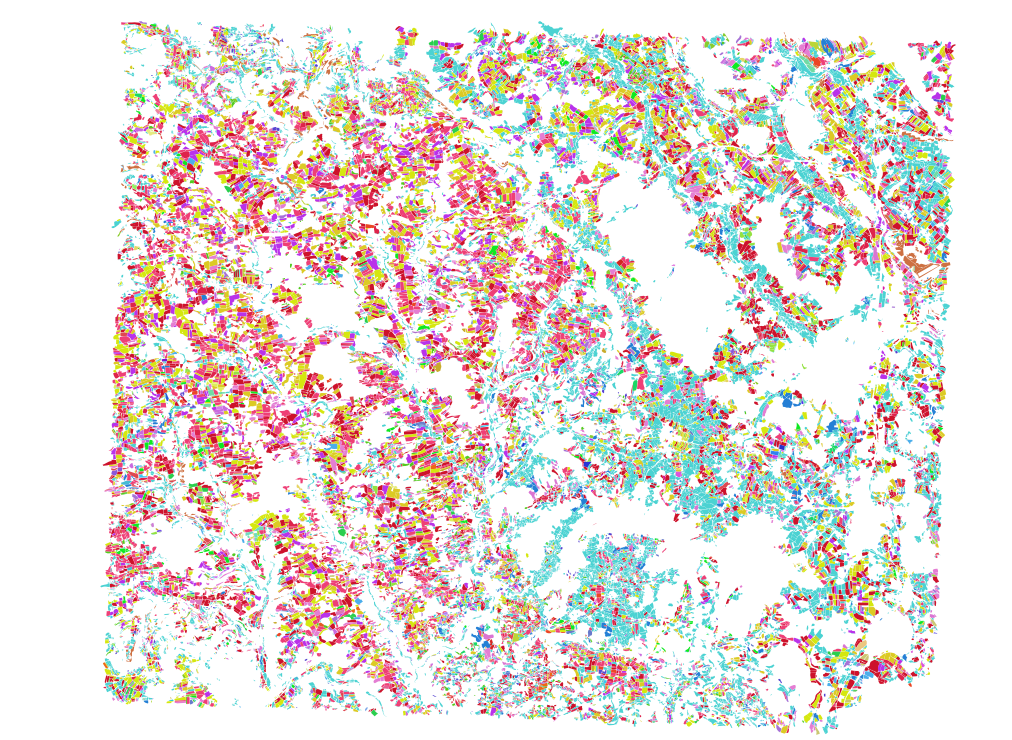
\includegraphics[width=\textwidth]{images/holl}
		\small
		Parcels colored by crop type (40 km by 40 km)
		
	\end{columns}
	
\end{frame}

\begin{frame}<presentation:7>
\frametitle{Two Datasets: Raw and Preprocessed from the same Examples}
%	
%	[format] in this presentation we have the special opportunity to to compare commercially pre-processed satellite imagery with raw imagery on crop type classification in Bavaria Germany.
%	
\begin{tikzpicture}[node distance=.1em]
\node[draw=black, rounded corners, minimum height=3cm, minimum width=4.5cm, label=below:preprocessing, font=\Large\bfseries](gaf){%
	\only<1>{
\includegraphics[width=2cm]{images/icons/gears}}%
	\only<2>{$f_{\Mweight_\text{sel}}$}%
	\only<3>{$f_{\Mweight_\text{sel}}\left(f_{\Mweight_\text{atm}}\right)$}%
	\only<4>{$f_{\Mweight_\text{sel}}\left(f_{\Mweight_\text{atm}}\left(f_{\Mweight_\text{cl}}\right)\right)$}%
	\only<5>{$f_{\Mweight_\text{sel}}\left(f_{\Mweight_\text{atm}}\left(f_{\Mweight_\text{cl}}\left(f_{\text{int}}\right)\right)\right)$}%
	\only<6>{$\Mweight_\text{preprocessing}$}%
	\only<7>{
\includegraphics[width=2cm]{images/GAF_logo}}%
};
\node[right=1.5em of gaf, inner sep=0](raw){\rawtimeseriestwo{12-71456800_raw.csv}};
\node[font=\huge,left=0em of raw, inner sep=0](bopen){$\Bigg($};
\node[font=\huge,right=0em of raw, inner sep=0](bopen){$\Bigg)$};
\visible<1->{
	\node[right=2em of raw, font=\huge](equals){$=$};
	\node[right=of equals, yshift=-1em](pre){\rawtimeseriestwo{12-71456800.csv}};
}
\only<7>{
\node[above=3em of raw, xshift=-2em](annotraw){raw data};
\node[above=4em of pre, xshift=2em](annotpre){preprocessed data};
\draw[-stealth] (annotraw) -- (raw);
\draw[-stealth] (annotpre) -- (pre);
}
\end{tikzpicture}

\only<1-6>{
	\begin{rdescription}
		\item[$f_{\Mweight_\text{sel}}(\M{X})$]<2-> temporal selection (not considering winter period) where $\Mweight_\text{sel} = \{t_\text{start}, t_\text{end}\}$
		\item[$f_{\Mweight_\text{atm}}(\M{X})$]<3-> atmospheric correction ($\M{X}_\text{top-of-atmosphere} \rightarrow \M{X}_\text{bottom-of-atmosphere}$)
		\item[$f_{\Mweight_\text{cl}}(\M{X})$]<4-> cloud/cloudshadow classification (F-Mask, MAJA, CNNs, Cloud Clustering (go FDL!))
		\item[$f_{\text{int}}(\M{X})$]<5-> temporal interpolation to generate equal sample times
		\item[$f_{\Mweight_\text{\dots}}$]<6-> many more...	
	\end{rdescription}
}
\only<7>{
	\vspace{2em}
	\centering\Large In this case: Preprocessing Engine of 
\includegraphics[width=4em]{images/GAF_logo}
}

\end{frame}

%\begin{frame}
%	\frametitle{Dataset}
%
%	
%	\begin{tikzpicture}[node distance=.5em]
%	\node(raw1){\rawtimeseriestwo{12-71456800_raw.csv}};
%	\node[right=of raw1](pre1){\rawtimeseriestwo{12-71456800.csv}};
%	
%	\node[below=of raw1](raw2){\rawtimeseriestwo{27-71460091_raw.csv}};
%	\node[right=of raw2](pre2){\rawtimeseriestwo{27-71460091.csv}};
%	
%	\node[above=of raw1]{Raw Sentinel 2 Data};
%	\node[above=of pre1]{
\includegraphics[width=1cm]{images/GAF_logo}-preprocessed Sentinel 2 Data};
%	
%	\node[left=of raw1]{meadow};
%	\node[left=of raw2]{wheat};
%	\end{tikzpicture}
%	
%%
%%\begin{tabular}{lcc}
%%	\toprule
%%	Datasets & Raw Sentinel 2 Data & 
\includegraphics[width=1cm]{images/GAF_logo}-preprocessed Sentinel 2 Data \\
%%	\cmidrule(lr){2-2}\cmidrule(lr){3-3}
%%	{\vspace{1em}meadow} &  & \rawtimeseriestwo{12-71456800.csv} \\
%%	{wheat} & \rawtimeseriestwo{27-71460091_raw.csv} & \rawtimeseriestwo{27-71460091.csv} \\
%%	{32 more} & \rawtimeseriestwo{1-71470174_raw.csv} & \rawtimeseriestwo{1-71470174.csv} \\
%%	\bottomrule
%%\end{tabular}
%
%%\begin{columns}[t]
%%	
%%	\column{.5\textwidth}
%%	Raw Sentinel 2 Data
%%	
%%	\rawtimeseriestwo{12-71456800_raw.csv}
%%	
%%	\column{.5\textwidth}
%%	
\includegraphics[width=2cm]{images/GAF_logo}-preprocessed Sentinel 2 Data
%%	
%%	\rawtimeseriestwo{12-71456800.csv}
%%	
%%\end{columns}
%
%%	\begin{tikzpicture}[baseline=-2em, inner sep=0]
%%
%%\begin{axis}[
%%thin,
%%width=6cm,
%%%hide axis,
%%height=3cm,
%%ymin=0, ymax=1.4,
%%no marks,  
%%draw opacity=.8,
%%smooth=0.01
%%]
%%%
%%%
%%\addplot[b11color] table [x=t, y=B11, col sep=comma, forget plot] {images/example/12-71456800_raw.csv};
%%\addplot[b12color] table [x=t, y=B12, col sep=comma] {images/example/12-71456800_raw.csv};
%%
%%\addplot[b5color] table [x=t, y=B05, col sep=comma, forget plot] {images/example/12-71456800_raw.csv};
%%\addplot[b6color] table [x=t, y=B06, col sep=comma, forget plot] {images/example/12-71456800_raw.csv};
%%\addplot[b7color] table [x=t, y=B07, col sep=comma, forget plot] {images/example/12-71456800_raw.csv};
%%\addplot[b8color] table [x=t, y=B08, col sep=comma, forget plot] {images/example/12-71456800_raw.csv};
%%\addplot[b8Acolor] table [x=t, y=B8A, col sep=comma] {images/example/12-71456800_raw.csv};
%%
%%\addplot[b2color] table [x=t, y=B02, col sep=comma, forget plot] {images/example/12-71456800_raw.csv};
%%\addplot[b3color] table [x=t, y=B03, col sep=comma, forget plot] {images/example/12-71456800_raw.csv};
%%\addplot[b4color] table [x=t, y=B04, col sep=comma] {images/example/12-71456800_raw.csv};
%%
%%\end{axis}
%%
%%\end{tikzpicture}
%\end{frame}


\begin{frame}
\frametitle{Four deep state-of-the-art Models for Time Series Classification}

\centering\begin{tabular}{lcccc}
	\toprule
	& LSTM-RNN$^1$ & Transformer$^1$ & MS-ResNet$^3$ & TempCNN$^4$ \\
	\cmidrule(lr){2-2}\cmidrule(lr){3-3}\cmidrule(lr){4-4}\cmidrule(lr){5-5}
	Mechanism & Recurrence & Self-Attention & Convolution & Convolution \\
	Parameter & 100k & 600k & 2Mio & 433k \\
	\bottomrule
\end{tabular}

\vspace{4em}

{\footnotesize\raggedright

$^1$ \textbf{Hochreiter, S., \& Schmidhuber, J. (1997)}. Long short-term memory. Neural computation, 9(8), 1735-1780.

$^2$ \textbf{Vaswani}, A., Shazeer, N., Parmar, N., Uszkoreit, J., Jones, L., Gomez, A. N., \& Polosukhin, I. \textbf{(2017)}. Attention is all you need. In Advances in neural information processing systems (pp. 5998-6008).

$^3$ \textbf{Wang}, F., Han, J., Zhang, S., He, X., \& Huang, D. \textbf{(2018)}. Csi-net: Unified human body characterization and action recognition. arXiv preprint arXiv:1810.03064.

$^4$ \textbf{Pelletier, C.}, Webb, G. I., \& Petitjean, F. \textbf{(2019)}. Temporal convolutional neural network for the classification of satellite image time series. Remote Sensing, 11(5), 523.

}

\end{frame}


\begin{frame}
\frametitle{Preprocessed versus Raw Data}

%\begin{tabular}{rrlrlrlrl}
%\toprule
%& \multicolumn{2}{c}{MS-ResNet$^1$} & \multicolumn{2}{c}{RNN (LSTM)$^2$} & \multicolumn{2}{c}{Transformer$^3$} & \multicolumn{2}{c}{TempCNN$^4$} \\
%& acc. & $\kappa$ & acc. & $\kappa$ & acc. & $\kappa$ & acc. & $\kappa$ \\
%\cmidrule(lr){2-3}\cmidrule(lr){4-5} \cmidrule(lr){6-7}\cmidrule(lr){8-9}
%\small pre & 0.80 $\pm$ 0.0035 & 0.76 $\pm$ 0.0042 & 0.80 $\pm$ 0.0019 & 0.76 $\pm$ 0.0028 & 0.85 $\pm$ 0.0039 & 0.81 $\pm$ 0.0046 & 0.84 $\pm$ 0.0012 & 0.80 $\pm$ 0.0016 \\
%\small raw & 0.80 $\pm$ 0.0026 & 0.75 $\pm$ 0.0032 & 0.83 $\pm$ 0.0038 & 0.80 $\pm$ 0.0043 & 0.83 $\pm$ 0.0038 & 0.80 $\pm$ 0.0043 & 0.80 $\pm$ 0.0025 & 0.75 $\pm$ 0.0032 \\
%
%%preprocessed & \textbf{0.8484} & \textbf{0.8150} & 0.8059 & 0.7616 & \textbf{0.8116} & \textbf{0.7680} & \textbf{0.8351} & \textbf{0.7971} \\
%%raw 		 & 0.8331 & 0.7971 & \textbf{0.8048} & \textbf{0.7611} & 0.7859 & 0.7420 & 0.7944 & 0.7462 \\
%\midrule
%& \\
%$\Delta$ & & & & \\
%\bottomrule
%\end{tabular}
{
\centering

\begin{tabular}{rccccc}
	\toprule
	\textbf{accuracy} & RNN (LSTM)$^2$ & Transformer$^3$ & MS-ResNet$^1$ & TempCNN$^4$ \\
	\cmidrule(lr){2-2}\cmidrule(lr){3-3} \cmidrule(lr){4-4}\cmidrule(lr){5-5}
	preprocessed & \textbf{.804} $^{\pm.0031}$ & .804 $^{\pm.0011}$ & \textbf{.849}$^{\pm .0041}$ & \textbf{.836} $^{\pm .0012}$ \\
	raw & .801 $^{\pm .0026}$ & \textbf{.842} $^{\pm .0043}$ & {.836} $^{\pm .0033}$ & .799 $^{\pm .0027}$ \\
	\midrule
	$\Delta$ & .003 $^{\pm .0041}$ & -.038 $^{\pm .0045}$ & .013 $^{\pm .0055}$ & .038 $^{\pm .0029}$ \\
	
	\bottomrule
\end{tabular}
\vspace{1em}

\begin{tabular}{rccccc}
	\toprule
	\textbf{kappa} & RNN (LSTM)$^2$ & Transformer$^3$ & MS-ResNet$^1$ & TempCNN$^4$ \\
	\cmidrule(lr){2-2}\cmidrule(lr){3-3} \cmidrule(lr){4-4}\cmidrule(lr){5-5}
	preprocessed & \textbf{.759} $^{\pm .0037}$ & .759 $^{\pm .0017}$ & \textbf{.816} $^{\pm .0048}$ & \textbf{.799} $^{\pm .0015}$ \\
	raw & .756 $^{\pm .0037}$ & \textbf{.808} $^{\pm .0052}$ & .800 $^{\pm .0039}$ & .750 $^{\pm .0036}$ \\
	\midrule
	$\Delta$ & .003 $^{\pm .0048}$ & -.049 $^{\pm .0054}$ & .016 $^{\pm .0060}$ & .049 $^{\pm .0036}$ \\
	
	\bottomrule
\end{tabular}

}
\vspace{1em}

\begin{columns}[t]
	\column{.5\textwidth}
	
	\textbf{Experiments}:
	\begin{itemize}
		\item mean $\pm$ standard deviation of 10 models trained from different random initialization
	\end{itemize}
	
	\column{.5\textwidth}
	
	\textbf{Findings}:
	\begin{itemize}
		\item preprocessed data seems slightly better except for transformer
		\item the difference $\Delta$ is only 0-5\%
	\end{itemize}
	

\end{columns}


\end{frame}
